\documentclass[10pt,a4paper]{article}
\usepackage[margin=2.4cm]{geometry}
\usepackage[T1]{fontenc}
\usepackage{lmodern}
\usepackage{microtype}
\usepackage{amsmath,amssymb}
\usepackage{graphicx}
\usepackage{booktabs}
\usepackage{tabularx}
\usepackage{array}
\usepackage{xcolor}
\usepackage{enumitem}
\usepackage[font=small,labelfont=bf]{caption}
\usepackage[authoryear,round]{natbib}
\usepackage[colorlinks=true,linkcolor=blue!50!black,citecolor=blue!50!black,urlcolor=blue!50!black]{hyperref}

\setlength{\parindent}{0pt}
\setlength{\parskip}{0.45em plus 0.1em}
\setlist{nosep,leftmargin=*,topsep=2pt}
\renewcommand{\arraystretch}{1.12}
\renewcommand{\bibfont}{\small}
\setlength{\bibsep}{1.5pt plus 0.5pt}

% --- conventions used throughout -------------------------------------------
\newcommand{\code}[1]{\texttt{\detokenize{#1}}}
\newcommand{\repo}{\par\textbf{In the repo.}\ }
\newcommand{\flag}{\textcolor{red!65!black}{\textbf{Flag.}}\ }
\newcommand{\unver}{\textcolor{orange!85!black}{\textbf{[unverified]}}}
\newcommand{\checked}{\textcolor{green!45!black}{\textbf{[checked numerically]}}}
\newcommand{\derived}{\textcolor{green!45!black}{\textbf{[derived here]}}}
\newcommand{\heur}{\textcolor{orange!85!black}{\textbf{[heuristic]}}}
\newcommand{\E}{\mathbb{E}}
\newcommand{\R}{\mathbb{R}}
\newcommand{\dd}{\,\mathrm{d}}
\newcommand{\nbar}{\bar n}

\title{\textbf{Point processes, summary functions and persistent homology}\\[3pt]
\large Working notes for the AISTATS submission}
\author{\normalsize point-process-tda, branch \texttt{frontend} at \texttt{6d5e0f3}}
\date{\normalsize 11 September 2026}

\begin{document}
\maketitle

\noindent\fbox{\parbox{\dimexpr\linewidth-2\fboxsep-2\fboxrule\relax}{\small
\textbf{How to read.} Each topic runs intuition $\to$ the equation(s) that matter $\to$ a figure where one helps.
\textbf{In the repo} paragraphs describe what the code does; paths are relative to \code{src/cloudforger/} unless they start with \code{configs/}, \code{scripts/}, \code{data/} or \code{docs/}.
\flag marks a departure from standard practice or a likely problem.
\checked{} marks a result compared against the repo's own simulators and estimators; \derived{} marks a derivation done for these notes; \unver{} marks a statement I could not verify; \heur{} marks an order-of-magnitude argument.
Every simulation-based number comes from SLURM job 26430628 (\code{sbatch docs/theory/scripts/theory_sims.sh}, then \code{python docs/theory/scripts/make_figures.py}); ``audit'' means \code{docs/status/audit.md}.
Conventions: window $W=[0,1]^2$, intensity $\lambda$ (expected points per unit area), $\nbar=\lambda|W|$, spacing $\ell=\lambda^{-1/2}$ (under CSR the mean nearest-neighbour distance is $\ell/2$), $b(u,r)$ the disc of radius $r$ at $u$.}}

% ============================================================================
\section{Why an encoder?}\label{sec:why}

A point pattern is an unordered set with a random number of points. Classical inference compresses it into hand-designed summaries ($K$, $G$, $F$) and then fits a model by matching them (minimum contrast, composite likelihood). A learned estimator replaces the matching step, and possibly the summaries too: a network trained on simulated (pattern, parameter) pairs learns the inverse map directly. This is amortised, likelihood-free inference. It helps when:
\begin{itemize}
  \item the map from summaries to parameters has no closed form or is badly conditioned (Strauss, nested clusters);
  \item the information is spread over many scales and several functions, which a fixed contrast weights poorly;
  \item inference has to be fast.
\end{itemize}
Representation learning exists to find task-relevant features rather than generic ones \citep{Bengio2013}.

In this project the encoder is the experimental unit. The prediction head is shared. What varies is the input representation (summary curves $L,F,G$ vs.\ vectorised persistence diagrams) and the encoder built for it. So ``topology adds information'' is really a claim about the best achievable encoder on each representation. Two consequences recur below:
\begin{enumerate}
  \item the encoder has to match the representation's geometry (\S\ref{sec:vec});
  \item everything else must be matched across arms, e.g.\ $n(x)$, budgets and optimisers; audit \S5.4 records where it currently is not.
\end{enumerate}

% ============================================================================
\section{Point processes}\label{sec:pp}

A quick reminder, with details in \S\ref{sec:sf}. The pair correlation $g(r)$ is the density of point pairs at distance $r$ relative to complete spatial randomness (CSR). Also $K(r)=2\pi\int_0^r s\,g(s)\dd s$ and $L=\sqrt{K/\pi}$; under CSR $g\equiv1$, $K=\pi r^2$ and $L=r$. For clustering two numbers summarise $g$:
\begin{itemize}
  \item its \emph{height}, $g(0)-1$;
  \item its \emph{mass}, $\lambda\int(g-1)$, the expected number of ``extra'' neighbours of a typical point.
\end{itemize}

\subsection{What a reviewer will expect}\label{sec:rank}

\begin{table}[ht]
\centering\small
\begin{tabularx}{\linewidth}{@{}l l X l@{}}
\toprule
 & Family & Why & Repo status\\
\midrule
Must & Poisson (CSR) & The null every summary is measured against; needed as a class and to calibrate a regime axis (\S\ref{sec:prop}). & simulator only\\
Must & Thomas & The canonical clustered model; closed-form $K$; the standard estimation benchmark. & data + results\\
Must & Strauss & The canonical regular (inhibitory) Gibbs model; the only regular process in the design. & data + results\\
Must$^\ast$ & Nested Thomas & Two cluster scales: the multiscale case that motivates persistent homology here. & data + results\\
Should & Mat\'ern cluster & Same mechanism with a compact kernel; tests kernel shape. The Thomas/Mat\'ern confusion is most of the classification difficulty. & data + results\\
Should & LGCP & The standard Cox model: a continuous random intensity with no discrete parents. & clouds only\\
Optional & Mat\'ern II & A second regular mechanism with closed-form $g$, but only weakly regular. & simulator only\\
Optional & Aniso.\ Thomas & Orientation, which rotation-invariant summaries cannot see by construction. & data + results\\
Optional & LGCP--Strauss & Regular at small $r$, clustered at large $r$ ($L-r$ changes sign). & clouds only\\
\bottomrule
\end{tabularx}
\caption{Families ranked by what an AISTATS reviewer will expect. $^\ast$Must for this paper's multiscale claim, not in general.}
\label{tab:rank}
\end{table}

\textbf{Design consequence.} CSR is absent from the classification bundle (\code{data/classification/classification_manifest.yaml}). Without a CSR class, the ``near-CSR'' stratum of \S\ref{sec:prop} has no null class to be confused with. Add it at matched $n$.

\subsection{Making difficulty comparable: dimensionless parameters}\label{sec:dimless}

Fix $\nbar$ and measure every length in units of $\ell$: $s=\sigma/\ell=\sigma\sqrt\lambda$ for a cluster scale and $\tau=R\sqrt\lambda$ for an interaction range. Each model then has one to three scale-free shape parameters, and $\nbar$ only sets the noise level. The repo's cluster designs use the \emph{overlap index} $c=2\sigma\sqrt\kappa$ (cluster diameter over parent spacing); for Thomas with $\mu=\lambda/\kappa$, $s=c\sqrt\mu/2$. Figure~\ref{fig:examples} shows one realization of each family at $\nbar=400$.

\begin{figure}[t]
\centering
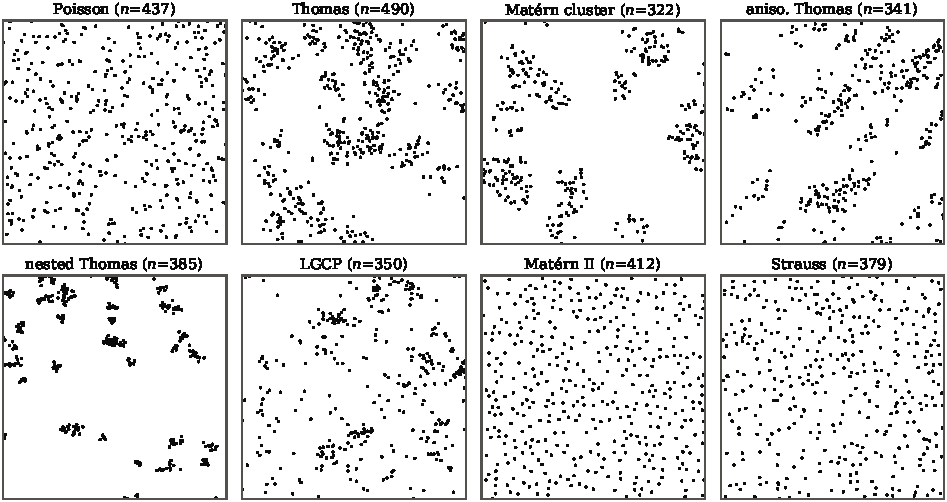
\includegraphics[width=\linewidth]{figs/fig_examples.pdf}
\caption{One realization per family, all at $\lambda=400$ on $[0,1]^2$, simulated with the repo's classes. Thomas: $\kappa=25$, $\sigma=0.04$. Mat\'ern cluster: its ``twin'' $R=2\sigma$. Aniso.\ Thomas: aspect 4, $\theta=\pi/4$. Nested: $\kappa=10$, $\mu_1=5$, $\sigma_1/\sigma_2=9$. LGCP: $\sigma^2=2$, $s=0.05$. Mat\'ern II: $R=0.025$. Strauss: $\beta=750$, $\gamma=0.2$, $R=0.025$.}
\label{fig:examples}
\end{figure}

\subsection{Poisson (CSR)}
\textbf{Intuition.} Points are dropped independently and uniformly; there is no interaction at any scale.
\textbf{Algorithm.} Draw $N\sim\mathrm{Poisson}(\lambda|W|)$, then $N$ i.i.d.\ uniform points. Conditioning on $N=n$ gives the binomial process used for Monte Carlo tests.
\textbf{Parameter.} $\lambda$ only.
\textbf{Closed forms.} $g=1$, $K=\pi r^2$, $L=r$, $G=F=1-e^{-\lambda\pi r^2}$, $J=1$.
\textbf{Sweep.} $\nbar\in\{100,200,400,800\}$; it serves as a reference, not an estimation target.
\repo \code{data_generation/point_processes/poisson.py}. With \code{intensity=None} it samples exactly $n$ points; the CSR null in these notes uses that.

\subsection{Neyman--Scott cluster processes: Thomas, Mat\'ern cluster, anisotropic Thomas}\label{sec:ns}
\textbf{Intuition.} Invisible \emph{parents} form a Poisson process of intensity $\kappa$. Each parent has a Poisson($\mu$) number of \emph{offspring}, scattered around it by a kernel; only the offspring are observed, so $\lambda=\kappa\mu$. The kernel is an isotropic Gaussian $N(0,\sigma^2I)$ for Thomas, uniform on a disc of radius $R$ for the Mat\'ern cluster process, and an elliptical Gaussian for anisotropic Thomas ($\sigma_{1,2}=\sigma a^{\pm1/2}$, angle $\theta$).
\textbf{Algorithm.}
\begin{enumerate}
  \item Place parents on $W$ dilated by a buffer, so that parents outside $W$ can still drop offspring inside.
  \item Draw offspring counts and displacements.
  \item Keep the offspring that fall in $W$.
\end{enumerate}
\textbf{Parameters.} $\kappa$ is the number of clusters, $\mu$ the cluster size and $\sigma$ (or $R$) the cluster extent.
\textbf{Closed forms} (derived in \S\ref{sec:derivK}):
\begin{equation}
K_{\rm Th}(r)=\pi r^2+\frac{1-e^{-r^2/(4\sigma^2)}}{\kappa},\qquad
K_{\rm MC}(r)=\pi r^2+\frac{D(r/R)}{\kappa},
\label{eq:Kns}
\end{equation}
where $D(d)=1+\tfrac{2}{\pi}(d^2-1)\arccos\tfrac d2-\tfrac d\pi\big(1+\tfrac{d^2}{2}\big)\sqrt{1-d^2/4}$ for $d\le2$ (and $1$ beyond) is the CDF of the distance between two uniform points in the unit disc \derived{}: differentiating it gives the disc-overlap density. For anisotropic Thomas, $K=\pi r^2+P(\|D\|\le r)/\kappa$ with $D\sim N(0,2\Sigma)$. That is a one-dimensional integral with no elementary form, and it does not depend on $\theta$ at all.
\textbf{Regimes.} Height and mass are $g(0)-1=1/(\pi c^2)$ and $\lambda\int(g-1)=\mu$. So $c$ alone sets how peaked the clustering is and $\mu$ sets how much of it there is. The process approaches CSR in three ways:
\begin{itemize}
  \item $c\to\infty$: clusters overlap and the random intensity flattens;
  \item $\mu\to0$ at fixed $\lambda$: each parent has at most one child;
  \item $\nbar\to0$: noise swamps everything.
\end{itemize}
A signal-to-noise index for $K$ follows from counting excess sibling pairs within $2\sigma$ against the Poisson fluctuation of all pairs: $D_{\rm Th}=\mu\sqrt{\nbar}/s=2\sqrt{\mu\nbar}/c$ \heur{}. On the current Thomas data its rank correlation with the observed departure statistic of \S\ref{sec:departure} is $0.94$.
\textbf{Twins.} The repo matches $R=2\sigma$ (\code{c1} in \code{matern_cluster.py}). This equalises the per-axis RMS displacement, and hence also $g(0)$ and the mass $1/\kappa$. The two $K$ curves then differ only through the kernel's tails and are almost indistinguishable (Fig.~\ref{fig:kfun}, Mat\'ern panel). That is the root of the Thomas/Mat\'ern confusion in classification.
\repo \code{neyman_scott.py:79-129}. The buffer is \code{Kernel.support_radius} (\code{kernels.py:73-78}): $\sigma\,\Phi^{-1}(1-10^{-4})\approx3.72\sigma$ for the Gaussian and exactly $R$ for the disc, so the omitted tail mass is $\le10^{-4}$ per axis. That is standard. \flag The design samples $(K,\mathrm{EN},c)$ log-uniformly (\code{configs/runs/thomas/*.yaml}). $\nbar$ therefore varies over $[150,800]$ (realised $n$ 51--1291, audit \S1.1), and difficulty is confounded with sample size. Moreover $c\le0.9$ keeps $g(0)-1\ge0.39$, so the design never approaches CSR (\S\ref{sec:departure}).

\subsection{Nested Thomas}\label{sec:nested}
\textbf{Intuition.} Clusters of clusters.
\textbf{Algorithm.}
\begin{enumerate}
  \item Meta-parents form a Poisson($\kappa$) process.
  \item Each meta-parent has Poisson($\mu_1$) parents displaced by $N(0,\sigma_1^2I)$.
  \item Each parent has Poisson($\mu_2$) offspring displaced by $N(0,\sigma_2^2I)$.
\end{enumerate}
So $\lambda=\kappa\mu_1\mu_2$.
\textbf{Closed form} (derived step by step in \S\ref{sec:derivK}):
\begin{equation}
K(r)=\pi r^2+\frac{1-e^{-r^2/(4\sigma_2^2)}}{\kappa\mu_1}+\frac{1-e^{-r^2/(4(\sigma_1^2+\sigma_2^2))}}{\kappa}.
\label{eq:Knested}
\end{equation}
There are two ``steps'': one near $r\approx2\sigma_2$ with mass $1/(\kappa\mu_1)$, one near $r\approx2(\sigma_1^2+\sigma_2^2)^{1/2}$ with mass $1/\kappa$.
\textbf{Regimes.}
\begin{itemize}
  \item $\sigma_1\to0$: collapses to Thomas with compound offspring (one step of mass $1/(\kappa\mu_1)+1/\kappa$).
  \item $\sigma_1\to\infty$: the parents become Poisson and the process becomes Thomas($\kappa\mu_1,\mu_2,\sigma_2$).
  \item It approaches CSR only when both levels dissolve.
\end{itemize}
The two scales are resolvable only if $\sigma_1/\sigma_2$ is well away from $1$; the repo constrains it to $[3,12]$.
\repo \code{nested_thomas.py:27-51}. The parent sampler is the Thomas meta-process, run on $W$ dilated by the inner buffer, and it adds its own outer buffer, so edges are handled correctly. The design axes are $c_1=2\sigma_1\sqrt\kappa$ and $c_2=2\sigma_2\sqrt{\kappa\mu_1}$ (each an overlap index at its own level). The repo's closed form (\code{baselines/mincontrast_nested.py:85-91}) matches (\ref{eq:Knested}); its docstring asks for independent checking, which \S\ref{sec:derivK} and Fig.~\ref{fig:kfun} now provide. \flag \code{configs/runs/nested_thomas/nested_thomas_vihrs.yaml} still carries a stale design block, with ranges unlike those in \code{fusion_k5.yaml}. Training reads \code{data/}, so this is harmless but misleading.

\subsection{Mat\'ern hard-core process (type II)}\label{sec:m2}
\textbf{Intuition.} Throw Poisson($\lambda_p$) candidates, each carrying a random ``age''. Delete every candidate that has an older neighbour within $R$. The survivors are at least $R$ apart.
\textbf{Parameters.} $(\lambda_p,R)$, with $\lambda=(1-e^{-\lambda_p\pi R^2})/(\pi R^2)<1/(\pi R^2)$.
\textbf{Pair correlation} \derived{}: $g(r)=0$ for $r<R$, and for $r\ge R$
\begin{equation}
g(r)=\frac{2\big[U(r)\,(1-e^{-\lambda_p\pi R^2})-\pi R^2\,(1-e^{-\lambda_pU(r)})\big]}{\lambda^2\,\pi R^2\,U(r)\,\big(U(r)-\pi R^2\big)},
\label{eq:m2}
\end{equation}
where $U(r)=|b(0,R)\cup b(re_1,R)|$. To derive it, note that two candidates with marks $m_1<m_2$ at distance $r\ge R$ both survive iff there is no candidate with mark $<m_1$ in the union of their discs and none with mark in $(m_1,m_2)$ in the second disc; then integrate over the marks. $K$ is a one-dimensional integral of (\ref{eq:m2}).
\textbf{Regimes.} It approaches CSR as $\tau=R\sqrt\lambda\to0$. Regularity is capped: $\tau<1/\sqrt\pi\approx0.56$ and the packing fraction is $\le1/4$, so Mat\'ern~II only covers mildly regular patterns.
\repo \code{data_generation/point_processes/matern.py:30-52}, registered as \code{matern}; it is in no current dataset. \flag Thinning happens inside $W$ only. Candidates just outside $W$, which would have deleted points near the edge, are never generated. Measured over 400 clouds, the intensity within $R$ of the boundary is $1.149\times$ the interior intensity and the mean $n$ is 406 against a theoretical 400. Thinning on $W\oplus R$ and cropping gives $0.998\times$ and 400 \checked{}.

\subsection{Strauss process}\label{sec:strauss}
\textbf{Intuition.} A Gibbs model in which every pair of points closer than $R$ costs a factor $\gamma\in[0,1]$. The density relative to a unit-rate Poisson process is $f(x)\propto\beta^{n(x)}\gamma^{s_R(x)}$, where $s_R$ counts the $R$-close pairs \citep{Strauss1975}. $\gamma=1$ gives Poisson($\beta$) and $\gamma=0$ a hard core. $\gamma>1$ is not integrable in the plane \citep{KellyRipley1976}, so Strauss cannot cluster.
\textbf{Algorithm.} Birth--death Metropolis--Hastings \citep{GeyerMoller1994}, driven by the Papangelou conditional intensity $\lambda(u\mid x)=\beta\gamma^{t(u,x)}$, where $t$ counts the points within $R$ of $u$. A birth at a uniform location is accepted with probability $\min\{1,\beta\gamma^{t}|W|/(n+1)\}$ and a death with the reciprocal ratio.
\textbf{Parameters.} $\beta$ is an \emph{activity}, not the intensity: $\lambda<\beta$, with no closed form, and there is no closed-form $g$ or $K$ either. A useful approximation treats the $R$-neighbours of a new point as Poisson($\lambda\pi R^2$), so $\E\gamma^t=e^{-\lambda G}$ with $G=(1-\gamma)\pi R^2$. Hence $\lambda=\beta e^{-\lambda G}$, i.e.\ $\lambda\approx W_0(\beta G)/G$ with $W_0$ the Lambert function, invertible as $\beta=\lambda e^{\lambda G}$. I believe this is the Poisson--saddlepoint approximation of \citet{BaddeleyNair2012} \unver{}. Against simulation it is within 1\% for weak or short-range inhibition, $+5\%$ at $\gamma=0.3$ and $+26\%$ at $\gamma=0.05$, $R=0.05$ (Table~\ref{tab:strauss}). It is a first guess for fixing $\nbar$; calibrate by simulation after it.
\textbf{Regimes.} It approaches CSR as $\gamma\to1$ or when $\pi\tau^2(1-\gamma)\to0$, i.e.\ when few pairs are ever within $R$. By analogy with Thomas, a signal index is $D_{\rm S}=\sqrt{\nbar}\,\tau(1-\gamma)$ \heur{}; its rank correlation with the observed departure on the current data is $0.91$.
\repo \code{gibbs.py:28-100,140-152}. The chain starts from Poisson($\beta$) on $W$ dilated by $2R$, runs $\max(15000,40\beta|W\oplus2R|)$ steps (about 40 sweeps), and is then clipped to $W$. The audit flagged convergence as unverified. Table~\ref{tab:strauss} compares that budget with $10\times$ it, 40 chains each: neither the mean $n$ nor the mean $\hat L-r$ moves beyond Monte Carlo error, including at $\gamma=0.05$, $R=0.05$ \checked{}. This is evidence that the default budget reaches equilibrium for these statistics, not a proof. \flag $\gamma$ and $R$ are sampled independently of $\beta$, and $R$ goes down to $0.005$ ($\tau\approx0.07$). As a result 28\% of Strauss clouds are indistinguishable from CSR by $L$ (\S\ref{sec:departure}), and on those $\gamma$ is at best weakly identified. That is a more likely contributor to the Strauss ``$\gamma$-gap'' than MH mixing, and it is testable: the $\gamma$ error should fall with $S_L$.

\begin{table}[ht]
\centering\small
\begin{tabular}{@{}l ccc cc c c@{}}
\toprule
 & & & & \multicolumn{2}{c}{mean $n$ (s.e.)} & & \\
\cmidrule(lr){5-6}
setting & $\beta$ & $\gamma$ & $R$ & $1\times$ & $10\times$ & PS & $\max_r|\Delta\hat L|$ / 2 s.e.\\
\midrule
weak     & 400 & 0.80 & 0.020 & 362.4 (2.9) & 368.6 (2.6) & 364.9 & 0.0005 / 0.0006\\
moderate & 600 & 0.30 & 0.030 & 300.6 (2.0) & 304.9 (2.0) & 319.1 & 0.0006 / 0.0008\\
strong   & 900 & 0.05 & 0.050 & 160.3 (1.2) & 159.4 (1.1) & 200.9 & 0.0017 / 0.0015\\
small $R$& 400 & 0.05 & 0.008 & 370.1 (2.8) & 368.7 (3.1) & 372.5 & 0.0005 / 0.0006\\
\bottomrule
\end{tabular}
\caption{Strauss: the repo's MH budget ($1\times$) against $10\times$, 40 chains each. PS is the approximation $W_0(\beta G)/G$. The last column is the largest difference between the two mean $\hat L-r$ curves on $r\le0.12$ against twice its standard error.}
\label{tab:strauss}
\end{table}

\subsection{Log-Gaussian Cox process (LGCP)}\label{sec:lgcp}
\textbf{Intuition.} Draw a random smooth ``heat map'' $\Lambda(u)=\exp Y(u)$, with $Y$ a Gaussian field, then scatter Poisson points according to it. Clustering is continuous: there are hot regions rather than discrete clusters \citep{Moller1998}.
\textbf{Algorithm.} Simulate $Y$ on $W$ (no buffer is needed), then thin a dominating Poisson process.
\textbf{Parameters.} $\mu$ is the log-mean, $\sigma^2$ the field variance (clustering strength) and $s$ the correlation length (clump size), with $\lambda=e^{\mu+\sigma^2/2}$.
\textbf{Closed forms.} For covariance $\sigma^2e^{-r/s}$, $g(r)=\exp(\sigma^2e^{-r/s})$. Expanding the exponential and integrating term by term gives \derived{}
\begin{equation}
K(r)=\pi r^2+2\pi\sum_{k\ge1}\frac{\sigma^{2k}}{k!}\Big(\frac sk\Big)^2\Big[1-\Big(1+\frac{kr}{s}\Big)e^{-kr/s}\Big].
\label{eq:Klgcp}
\end{equation}
\textbf{Regimes.} It approaches CSR as $\sigma^2\to0$, and also as $s\sqrt\lambda\to0$: the field decorrelates below the point spacing. $g(0)=e^{\sigma^2}$ stays large, but the mass $\lambda\int(g-1)\propto\lambda s^2\to0$. When $s$ is comparable to $W$, a single window sees one smooth trend. The pattern then looks like an inhomogeneous Poisson process, and $\hat K$ is unstable (non-ergodic in $W$).
\repo \code{cox.py:29-92,138-158}. The field is built from 512 random Fourier features \citep{RahimiRecht2007}, with Cauchy frequencies for the exponential covariance; that is correct in distribution as the number of features grows. Thinning uses a bound set by the maximum of the field over 8192 probe points plus $0.5$, and points above the bound are kept with probability one. \flag Both are approximations. The check in Fig.~\ref{fig:kfun} passes, with a caveat: normalised by the true $\lambda$, the simulated $K$ sits $1.7$ Monte Carlo s.e.\ below (\ref{eq:Klgcp}) at every $r$, and the mean count is $396$ against $400$ ($-1.5$ s.e.). With the repo's $n(n-1)$ normalisation the gap disappears. So $g$ is right, and the small deficit is in the count, which is where a thinning cap would act; it is not conclusive. LGCP has clouds but no diagrams or results.

\subsection{Recommended sweeps}\label{sec:sweeps}
Sample the dimensionless axes of Table~\ref{tab:sweeps} log-uniformly (linearly for $\gamma$) at fixed $\nbar$. Treat $\nbar\in\{200,400,800\}$ as a separate factor, not a nuisance, and map back to model parameters. The ranges deliberately \emph{include} the CSR limit, which the current designs miss (\S\ref{sec:departure}). Report every result against the population departure $S^\ast$ of \S\ref{sec:departure}, so that ``hard'' means the same thing for every process.

\begin{table}[ht]
\centering\small
\begin{tabularx}{\linewidth}{@{}l l X l@{}}
\toprule
Process & Axes & Range & Map back\\
\midrule
Thomas & $s=\sigma\sqrt\lambda$, $\mu$ & $s\in[0.1,3]$, $\mu\in[1.5,40]$ ($c$ up to $\approx5$, i.e.\ $g(0)-1\approx0.01$) & $\kappa=\lambda/\mu$, $\sigma=s\ell$\\
Mat\'ern cluster & $s$, $\mu$ & as Thomas, twin-matched & $R=2s\ell$\\
Nested Thomas & $s_2$, $\rho=\sigma_1/\sigma_2$, $\mu_1$, $\mu_2$ & $s_2\in[0.1,1]$, $\rho\in[3,12]$, $\mu_1\in[1.5,8]$, $\mu_2\in[1.5,20]$; reject $\kappa|W|<3$ & $\kappa=\lambda/(\mu_1\mu_2)$\\
Mat\'ern II & $\tau=R\sqrt\lambda$ & $[0.05,0.55]$ & $\lambda_p=-\ln(1-\pi\tau^2)/(\pi R^2)$\\
Strauss & $\tau$, $\gamma$ & $\tau\in[0.1,1]$, $\gamma\in[0,1)$ & $\beta\approx\lambda e^{(1-\gamma)\pi\tau^2}$, then calibrate\\
LGCP & $\sigma^2$, $s\sqrt\lambda$ & $\sigma^2\in[0.1,3]$, $s\sqrt\lambda\in[0.5,5]$ & $\mu=\ln\lambda-\sigma^2/2$\\
\bottomrule
\end{tabularx}
\caption{Recommended sweeps in dimensionless coordinates at fixed $\nbar$. The ranges cover the CSR limit of every family.}
\label{tab:sweeps}
\end{table}

% ============================================================================
\section{Summary functions}\label{sec:sf}

Second-order quantities describe pairs of points. The \emph{product density} $\rho^{(2)}(u,v)$ is the probability of finding points in two small discs at $u$ and $v$, per unit area squared. For a stationary, isotropic process $\rho^{(2)}(u,v)=\lambda^2g(\|u-v\|)$, so $g>1$ means attraction and $g<1$ inhibition. Table~\ref{tab:sf} lists the functions; the paragraphs after it add what the table cannot hold.

\begin{table}[ht]
\centering\small
\begin{tabularx}{\linewidth}{@{}l X X l@{}}
\toprule
 & Question it answers & Estimator (edge correction) & CSR value\\
\midrule
$K(r)$ & How many further points lie within $r$ of a typical point ($\times\lambda^{-1}$), cumulatively over scales? & $\frac{|W|}{n(n-1)}\sum_{i\ne j}w_{ij}\mathbf 1\{d_{ij}\le r\}$; Ripley isotropic $w_{ij}$ & $\pi r^2$\\
$L(r)$ & The same on a distance scale; $L-r$ removes the CSR trend and roughly stabilises the variance. & $\sqrt{\hat K/\pi}$ & $r$\\
$g(r)$ & Neighbour density at exactly distance $r$ (non-cumulative $K'$). & kernel-smoothed pair distances & $1$\\
$G(r)$ & Is the nearest other point of a typical point within $r$? (short-range clumping vs.\ inhibition) & reduced sample (border) & $1-e^{-\lambda\pi r^2}$\\
$F(r)$ & Is the nearest point of a \emph{fixed location} within $r$? (voids, empty space) & reduced sample on a test grid & $1-e^{-\lambda\pi r^2}$\\
$J(r)$ & $(1-G)/(1-F)$: $J<1$ clustering, $J>1$ regularity, not second-order. & ratio of the two & $1$\\
\bottomrule
\end{tabularx}
\caption{The six summary functions.}
\label{tab:sf}
\end{table}

\textbf{$K$ and $L$.} $K$ sees only pairs. Different processes can share $K$; there is even a non-Poisson process with the $K$ of CSR \citep{BaddeleySilverman1984}. Ripley's isotropic weight is $w_{ij}=2\pi d_{ij}/\mathrm{length}(\partial b(x_i,d_{ij})\cap W)$ \citep{Ripley1977}: the inverse fraction of the circle through $x_j$ centred at $x_i$ that lies inside $W$. $L-r$ is the version people plot and feed to networks.
\textbf{$G$, $F$, $J$.} These depend on the whole distribution, not just on pairs: $F$ is a void probability and $G$ a void probability seen from a typical point. $F$ probes empty space, which matters for clusters with gaps between them. $G$ probes the nearest-neighbour scale, where inhibition acts. $J$ combines them into a statistic that is identically $1$ for Poisson \citep{vanLieshoutBaddeley1996}. Standard estimators and edge corrections are in \citet{Diggle2013}, \citet{Illian2008} and \citet{Baddeley2015}; the reduced-sample estimator keeps only points (or test locations) farther than $r$ from the boundary.

\repo $L-r$: \code{baselines/vihrs.py:163-226}. It uses the isotropic correction with closed-form rectangle arcs and $\hat\lambda^2=n(n-1)/|W|^2$, on \code{linspace(0,0.25,513)}. $G$ and $F$: \code{baselines/summstats.py:78-155}. These are reduced-sample estimators on the same grid, with $F$ evaluated on a $64\times64$ interior grid of test locations. $J$ (\code{:158-184}) is held flat once $1-F<0.05$ and clipped at 5. Curves enter the vihrs CNN as channels (\code{vihrs.py:414-448}: Conv1d(64,7)--pool5 twice, then Conv1d, concatenated with $\log n$, then Dense 64--32). Each channel gets one pooled $z$-score over all training clouds and radii (\code{:381-402}). In \code{pi_multik}, $L$ ($F$, $G$) can also enter as 8--16 log-spaced side columns, or as full curves through a copy of that trunk.
\flag \code{summstats.py:117} enforces monotonicity with a cumulative max, which biases $\hat G$, $\hat F$ slightly upwards; spatstat does not do this. The module docstring calls the reduced-sample estimator ``exactly unbiased''; it is \emph{ratio}-unbiased.
\flag The shared grid wastes most of $G$: under CSR, $G\ge0.99$ beyond $r=\sqrt{\ln100/(\pi\lambda)}$, which is 60\%, 76\% and 83\% of $[0,0.25]$ at $\lambda=150,400,800$, and clustered patterns saturate earlier still. A grid in units of $\hat\ell=n^{-1/2}$ (say $r\sqrt n\in[0,3]$) would give every cloud the same resolution where $G$ and $F$ vary.
\flag \code{baselines/mincontrast.py:30-55} crops clouds with $n>900$ to a sub-window of side $w=\sqrt{900/n}$ and rescales it to the unit square. \code{scripts/train.py:409} then scores $\hat\kappa,\hat\sigma$ in the rescaled frame, never mapping them back ($\kappa=\hat\kappa/w^2$, $\sigma=\hat\sigma w$). This affects the $n>900$ tail of the min-contrast baseline.

\subsection{\texorpdfstring{Deriving $K$}{Deriving K}}\label{sec:derivK}

\textbf{General.} The second-order factorial moment measure is $\alpha^{(2)}(A\times B)=\E\sum^{\ne}_{x,y\in X}\mathbf 1\{x\in A,y\in B\}=\int_A\int_B\rho^{(2)}(u,v)\dd u\dd v$. Define $\lambda K(r)$ as the expected number of further points within $r$ of a typical point, a Palm expectation. By the Campbell--Mecke formula,
\begin{equation}
\begin{split}
\lambda|W|\cdot\lambda K(r)&=\E\sum^{\ne}_{x,y}\mathbf 1\{x\in W,\ \|y-x\|\le r\}\\
&=\int_W\int_{b(u,r)}\lambda^2g(\|v-u\|)\dd v\dd u=\lambda^2|W|\int_{b(0,r)}g,
\end{split}
\label{eq:campbell}
\end{equation}
so $K(r)=\int_{b(0,r)}g=2\pi\int_0^rs\,g(s)\dd s$ \citep{MollerWaagepetersen2003}. The estimator in Table~\ref{tab:sf} is (\ref{eq:campbell}) read backwards. Replace the expectation by the observed sum over pairs in $W$, reweight each pair to account for the unseen part of $b(x_i,d_{ij})$, and replace $\lambda^2$ by $\hat\lambda^2$.

\textbf{Neyman--Scott.} Classify ordered pairs of distinct points by whether they share a parent. Pairs with different parents come from independent clusters of a Poisson parent process, whose product density is $\kappa^2$, so they contribute $(\kappa\mu)^2=\lambda^2$. Pairs with the same parent contribute
$\kappa\,\E[N(N-1)]\int k(u-c)\,k(v-c)\dd c=\kappa\mu^2\,\tilde k(u-v)$,
where $\tilde k$ is the density of $D-D'$ for two independent displacements and $\E N(N-1)=\mu^2$ for Poisson counts. Therefore
\begin{equation}
g(r)=1+\tilde k(r)/\kappa,\qquad K(r)=\pi r^2+P(\|D-D'\|\le r)/\kappa .
\label{eq:gns}
\end{equation}
For Thomas, $D-D'\sim N(0,2\sigma^2I)$, so $\|D-D'\|^2/(2\sigma^2)\sim\chi^2_2$ and $P=1-e^{-r^2/(4\sigma^2)}$. This gives (\ref{eq:Kns}), and the mass is $\lambda\int(g-1)=\lambda/\kappa=\mu$.

\textbf{Nested Thomas, step by step} \derived{}.
\begin{enumerate}
\item \emph{Ancestry.} Every point has one parent and one meta-parent. An ordered pair of distinct points either (a) shares a parent; (b) shares a meta-parent but has different parents; or (c) has different meta-parents.
\item \emph{(c) gives $\lambda^2$.} Meta-parents form a Poisson($\kappa$) process and their family trees are independent, exactly as for different Neyman--Scott clusters.
\item \emph{(a).} Parents have intensity $\kappa\mu_1$. Each has $\E N_2(N_2-1)=\mu_2^2$ ordered offspring pairs, whose difference is $V-V'\sim N(0,2\sigma_2^2I)$. Contribution: $\kappa\mu_1\mu_2^2\,\varphi_{2\sigma_2^2}(u-v)$, where $\varphi_s$ is the $N(0,sI)$ density.
\item \emph{(b).} Each meta-parent has $\E N_1(N_1-1)=\mu_1^2$ ordered pairs of distinct parents, each giving $\mu_2\cdot\mu_2$ offspring pairs. The difference is $(U-U')+(V-V')\sim N(0,2(\sigma_1^2+\sigma_2^2)I)$. Contribution: $\kappa\mu_1^2\mu_2^2\,\varphi_{2(\sigma_1^2+\sigma_2^2)}(u-v)$.
\item \emph{Normalise} by $\lambda^2=\kappa^2\mu_1^2\mu_2^2$: $g(r)=1+\varphi_{2\sigma_2^2}(r)/(\kappa\mu_1)+\varphi_{2(\sigma_1^2+\sigma_2^2)}(r)/\kappa$.
\item \emph{Integrate} over $b(0,r)$, using $\int_{b(0,r)}\varphi_s=1-e^{-r^2/(2s)}$, to obtain (\ref{eq:Knested}).
\item \emph{Check.} Letting $\sigma_1\to0$ gives a Thomas process whose offspring count is compound Poisson. Its $\E N(N-1)/(\kappa(\E N)^2)=1/(\kappa\mu_1)+1/\kappa$ is the combined step mass, as it should be.
\end{enumerate}

\begin{figure}[t]
\centering
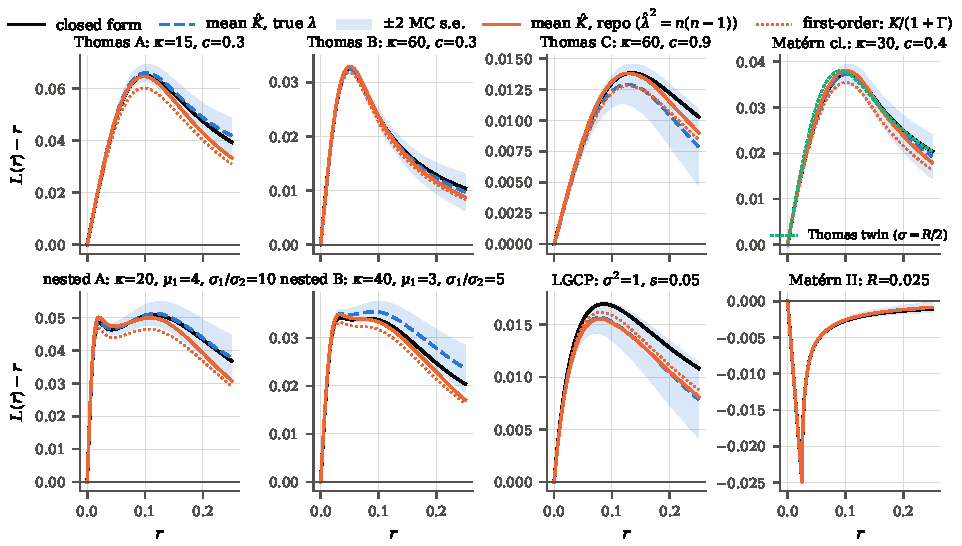
\includegraphics[width=\linewidth]{figs/fig_kfun.pdf}
\caption{Closed forms against the repo's simulators and its $L$ estimator: 400 clouds per panel, $\lambda=400$ (so $\mu=400/\kappa$). Curves are $L-r$ of the \emph{mean} $\hat K$ (no Jensen gap). Blue dashed: the true $\lambda$ is used in $\hat K$; the band is $\pm2$ Monte Carlo s.e. Orange: the repo's $\hat\lambda^2=n(n-1)$. Dotted: the first-order prediction $K/(1+\Gamma)$. The Mat\'ern panel adds the closed form of its Thomas twin ($\sigma=R/2$). Mat\'ern II is simulated on $W\oplus R$ (\S\ref{sec:m2}).}
\label{fig:kfun}
\end{figure}

\textbf{Numerical check} \checked{} (Fig.~\ref{fig:kfun}). The eight settings are Thomas $\times3$, Mat\'ern cluster, nested $\times2$, LGCP and Mat\'ern~II, each estimated with the repo's \code{_isotropic_l_minus_r} and normalised by the true $\lambda$. Pointwise, the mean $\hat K$ is within $1.9$ Monte Carlo s.e.\ of the closed form at every $r\in[0.01,0.25]$ in every setting. The curves are cumulative, so the deviations across $r$ are strongly correlated; a steady $z\approx-1.7$ (LGCP) or $+1.5$ (nested B) is one fluctuation, not many. So (\ref{eq:Kns})--(\ref{eq:Klgcp}) are right, and the repo's simulators produce the processes they claim to, with the LGCP caveat of \S\ref{sec:lgcp}.

\textbf{A bias the check exposed: $\hat\lambda^2$ absorbs clustering} \derived{}.
Clustering makes $n$ over-dispersed, so $\E[n(n-1)]=\lambda^2|W|^2(1+\Gamma)$, with $\Gamma=|W|^{-2}\int\gamma_W(h)(g(h)-1)\dd h\approx1/\kappa$ for Neyman--Scott processes. Here $\gamma_W(h)=|W\cap(W+h)|$; on the unit square, averaged over directions, it is $1-4r/\pi+r^2/\pi$. To first order, $\E\hat K(r)\approx K(r)/(1+\Gamma)$: part of the clustering is explained away as a high intensity. In the orange curves, at $r=0.25$ the repo's $\hat L-r$ sits 12--25\% below the population value. The first-order formula gets the size right (the observed shift is 0.6--1.3 times the prediction); the rest is the ratio's second-order term, since $\mathrm{CV}(n)$ reaches 0.25. This is harmless for a network trained on the same estimator, which learns the bias. It does bias minimum contrast against the closed forms (the repo's min-contrast uses $\hat\lambda=n$, translation correction, \code{mincontrast.py:58-86}), and it shrinks departure measures when $\kappa$ is small. On the current data that shrinkage is small: the observed-to-population ratio of $S_L$ has median 0.99 (\S\ref{sec:departure}).

\subsection{\texorpdfstring{Why $G$ and $F$ have no closed form (and where they almost do)}{Why G and F have no closed form}}\label{sec:GF}
$F$ is a void probability, $1-F(r)=P(X\cap b(0,r)=\emptyset)$, and $G$ is the same probability under the Palm distribution. Both need the whole distribution of $X$ (all orders of moments), which is available only through a generating functional. Where that functional is explicit, one gets integrals rather than closed forms. For Neyman--Scott processes with Poisson($\mu$) offspring \derived{}:
\begin{equation}
\begin{aligned}
1-F(r)&=\exp\Big(-\kappa\int_{\R^2}\big(1-e^{-\mu\,p_r(y)}\big)\dd y\Big),\\
J(r)&=\E\,e^{-\mu\,p_r(D)},\qquad 1-G(r)=J(r)\,\big(1-F(r)\big),
\end{aligned}
\label{eq:FGJ}
\end{equation}
with $p_r(y)=P(y+D\in b(0,r))$ and $D\sim k$.
\begin{itemize}
  \item The first identity is the Poisson generating functional applied to the cluster void probabilities.
  \item For the other two: the Palm distribution of the typical point is the process plus its siblings. The siblings form a Poisson process with intensity $\mu k(\cdot+D)$ (a size-biased Poisson minus one is Poisson), and $J$ is the probability that none of them lies within $r$.
\end{itemize}
For Thomas, $p_r$ is a non-central $\chi^2_2$ CDF, so (\ref{eq:FGJ}) is a set of one-dimensional integrals. Against the repo's estimators they agree to within $0.016$ for $F$ and $0.007$ for $G$ on the CDF scale, and to $0.04$ for $J$ up to $r=0.06$ \checked{} (Fig.~\ref{fig:checks}a--c). \citet{vanLieshoutBaddeley1996} give $J$ for Poisson cluster processes.

Beyond this family:
\begin{itemize}
  \item \emph{Nested Thomas}: nested generating functionals, which lead to two-dimensional integrals.
  \item \emph{LGCP}: $F$ needs the Laplace transform of an integral of a lognormal field, which has no closed form.
  \item \emph{Mat\'ern II}: nothing tractable beyond $g$.
  \item \emph{Strauss}: not even $\lambda$.
\end{itemize}

\begin{figure}[t]
\centering
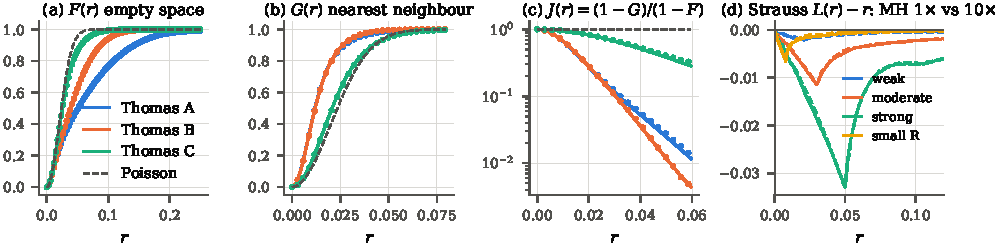
\includegraphics[width=\linewidth]{figs/fig_checks.pdf}
\caption{(a--c) The Thomas integrals (\ref{eq:FGJ}) (lines) against the mean of the repo's reduced-sample estimators (dots) over 400 clouds per setting of Fig.~\ref{fig:kfun}; the Poisson reference is dashed. (d) Strauss mean $\hat L-r$ with the repo's MH budget (solid) and $10\times$ it (dashed), 40 chains each (Table~\ref{tab:strauss}).}
\label{fig:checks}
\end{figure}

% ============================================================================
\section{Persistent homology for point clouds}\label{sec:ph}

\subsection{\texorpdfstring{Filtrations, diagrams, and what $H_0$ and $H_1$ see}{Filtrations, diagrams, and what H0 and H1 see}}\label{sec:filt}

\textbf{Intuition.} Grow a disc around every point and watch the union as the radius increases. Components ($H_0$) merge and loops ($H_1$) open and fill in. Each feature is born at some scale $b$ and dies at $d$, and the multiset of points $(b,d)$ is the persistence diagram. The \emph{Rips} filtration encodes this combinatorially: a simplex enters when all its pairwise distances are $\le t$ (ripser's diameter convention).
\begin{itemize}
  \item \textbf{$H_0$ under Rips.} Every point is born at $0$. Components merge at the single-linkage heights, which are exactly the minimum-spanning-tree (MST) edge lengths: ripser's finite $H_0$ deaths equal the MST edges to $6\times10^{-9}$ \checked{}. Every nearest-neighbour edge belongs to the MST; under CSR 69\% of MST edges are nearest-neighbour edges (100 clouds, $n=400$) \checked{}. So Rips-$H_0$ is essentially $G$ at small scales plus the gaps between clusters at large scales.
  \item \textbf{$H_1$.} A loop is born when a ring of points closes around an empty region and dies when triangles fill it. In clustered patterns the long-lived loops are the voids between clusters, which relates them to $F$. Under CSR, $H_1$ is many short-lived loops. In the example of Fig.~\ref{fig:ph}, the Thomas cloud has 37 DTM-$H_1$ points with maximum persistence 0.099; CSR at the same $n$ has 65, with maximum 0.067.
\end{itemize}
\textbf{Diagrams are statistics.} For stationary processes the diagram, normalised by $|W|$, converges to a deterministic measure on the $(b,d)$ plane \citep{Hiraoka2018}. So vectorisations estimate population functionals, just as $\hat K$ does, and they have the same issues of variance, edge effects and dependence on $n$. \citet{BiscioMoller2019} use persistent homology summaries for exactly this purpose: model checking with global envelopes.

\textbf{DTM filtration.} Replace ``distance to the nearest point'' by the \emph{distance to measure} \citep{ChazalCohenSteinerMerigot2011}:
\begin{equation}
\mathrm{DTM}_k(x)=\Big(\frac1k\sum_{j=1}^{k}\|x-X_{(j)}(x)\|^2\Big)^{1/2},
\qquad \E\,\mathrm{DTM}_k^2=\frac{k-1}{2\pi\lambda}\ \text{under CSR}.
\label{eq:dtm}
\end{equation}
The sum runs over the $k$ nearest data points, and gudhi counts $x$ itself as the first of them. The expectation follows because $\pi\lambda D_j^2\sim\mathrm{Gamma}(j,1)$ for the $j$-th nearest-neighbour distance \derived{}; interior points give $1.584\times10^{-3}$ against the predicted $1.592\times10^{-3}$ \checked{}. So $\mathrm{DTM}_k$ is a smoothed inverse local density. The weighted-Rips construction of \citet{Anai2020} ($p=1$) lets vertex $x$ enter at $2\,\mathrm{DTM}(x)$ (gudhi doubles every value) and edge $xy$ at $\|x-y\|+\mathrm{DTM}(x)+\mathrm{DTM}(y)$. Dense points enter early and isolated ones late. The $H_0$ diagram becomes a cluster tree of a $k$-NN density: a point $(b,d)$ is a cluster whose core density is about $b^{-2}$ and which merges into a denser one at $d$.

\textbf{What $k$ does.} $k$ sets the mass ($k/n$) over which density is averaged. Small $k$ resolves small clusters but is noisy. Large $k$ smooths away clusters of fewer than about $k$ points and suppresses outliers. Keep $k\lesssim\mu$ to see individual clusters. The design has $\mu$ down to 2.5, so at $k=5$ the smallest clusters are already invisible to $H_0$ births.

\textbf{Stability.} Diagrams are 1-Lipschitz in the bottleneck distance with respect to sup-norm perturbations of the filtration \citep{CohenSteiner2007}. For Rips on point clouds this makes them stable in Hausdorff distance \citep{ChazalMichel2021}, but a single outlier can move the Hausdorff distance a lot. DTM filtrations are stable with respect to Wasserstein distances between empirical measures \citep{Anai2020}, i.e.\ robust to outliers and noise points. That is the principled reason to prefer DTM for point processes.

\repo \code{data_generation/filtration/rips.py:31-36} (ripser, $H_0$ and $H_1$) and \code{dtm.py:62-82} (gudhi \code{DTMRipsComplex}, $q=2$ being the DTM exponent). Diagrams exist for $k\in\{5,10,15\}$ and Rips. Every vectoriser drops the infinite $H_0$ bar (\code{core/diagram.py:24-30}); under Rips it carries nothing, and under DTM only $\min\mathrm{DTM}$. I confirmed that the saved DTM $H_0$ births equal $2\,\mathrm{DTM}_5$ exactly.

\subsection{\texorpdfstring{The Rips-$H_0$ degeneracy}{The Rips-H0 degeneracy}}\label{sec:degenerate}
Under Rips every $H_0$ birth is $0$, so the $H_0$ diagram is one-dimensional: a multiset of $n-1$ deaths. Any vectorisation with a birth axis collapses. The repo's persistence-image calibration raises (\code{calibration/diagram_calibration.py:115-116}), and the ``1-D fallback'' described in the writeup does not exist (audit~\S2). Three remedies:
\begin{enumerate}
  \item Vectorise the deaths only: a 1-D density or histogram, or $\beta_0(t)=\#\{\text{MST edges}>t\}$. This loses nothing.
  \item Use DTM, whose births carry local density.
  \item Report Rips-$H_0$ as ``not meaningful'' for persistence images, as the audit does.
\end{enumerate}
Whichever you choose, remember that Rips-$H_0$ always contains $n$ exactly and overlaps heavily with $G$. Its only extra content is the large MST edges.

\begin{figure}[t]
\centering
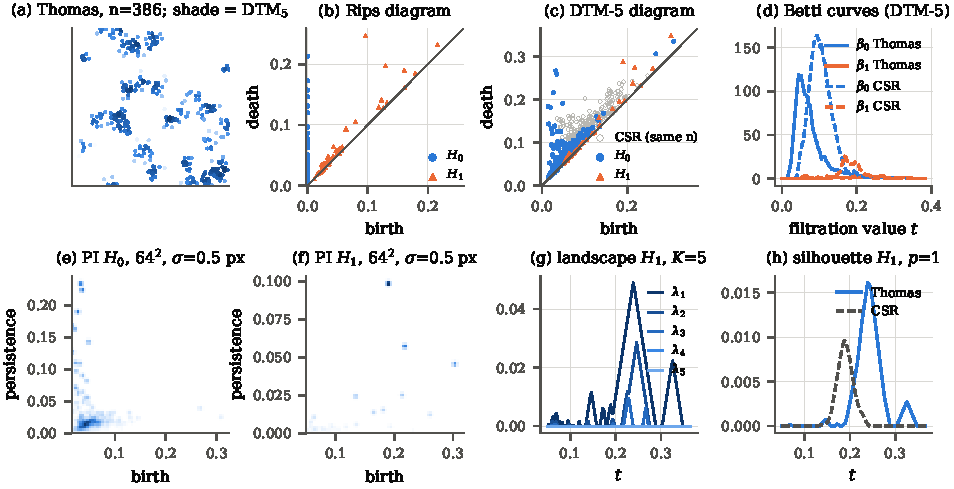
\includegraphics[width=\linewidth]{figs/fig_ph.pdf}
\caption{One Thomas cloud ($\kappa=30$, $c=0.35$, $n=386$) through the pipeline, using the repo's classes. (a) Points shaded by $\mathrm{DTM}_5$ (darker is denser). (b) Rips diagram: all $H_0$ points sit at birth $0$. (c) DTM-5 diagram, with a CSR cloud of the same $n$ in grey. (d) Betti curves, Thomas solid and CSR dashed. (e, f) Persistence images at the repo's settings ($64^2$, $\sigma=0.5$\,px; box fitted to these two diagrams). (g) First five landscapes of DTM-$H_1$. (h) Silhouettes, $p=1$.}
\label{fig:ph}
\end{figure}

\subsection{Vectorisations and the encoder each deserves}\label{sec:vec}
For each vectorisation below: construction, hyperparameters, stability, what it loses, and the encoder that suits it. Table~\ref{tab:vec} summarises.

\textbf{Persistence images} \citep{Adams2017}.
\begin{itemize}
  \item \emph{Construction.} Map $(b,d)\mapsto(b,p)$ with $p=d-b$, place a Gaussian of width $\sigma$ on each point weighted by $w(p)$ (linear, $w=p$), and integrate over a pixel grid on a fixed box.
  \item \emph{Hyperparameters.} The box, the resolution, $\sigma$ and $w$.
  \item \emph{Stability.} Lipschitz with respect to the 1-Wasserstein distance between diagrams, with a constant that grows like $1/\sigma$; it needs $w(0)=0$.
  \item \emph{Loses.} Structure finer than $\sigma$; mass outside the box; and short bars, through the weight. For point patterns the short bars are most of $H_0$ (the nearest-neighbour distances).
  \item \emph{Encoder.} The signal is \emph{where} the mass sits, so translation invariance is the wrong inductive bias. A CNN ending in global average pooling needs coordinate channels \citep{Liu2018coordconv}, or use a flatten/MLP head on a coarse image.
\end{itemize}
\repo \code{vectorization/persistence_images/persistence_image.py:25-109}. The repo uses exact pixel integrals, a $64^2$ grid and $\sigma=0.5$\,px, with the box fitted at coverage $q=0.95$ per seed, $k$ and dimension on training rows (\code{pi_multik.py:870-873}). Mass outside the box is lost, not clipped. The encoder is CoordConv 32/64/128 followed by global average pooling (\code{encoders/coordconv_pi.py:11-55}). \flag At $\sigma=0.5$\,px the image is a weighted histogram. In the example of Fig.~\ref{fig:ph}f, the DTM-$H_1$ image is 37 isolated one-pixel blobs among 4096 pixels: high-variance, sparse input. Try $\sigma\approx1$--$2$\,px, or $32^2$.

\textbf{Betti curves.}
\begin{itemize}
  \item \emph{Construction.} $\beta_k(t)=\#\{(b,d):b\le t<d\}$ on a grid; the Euler curve is $\chi=\beta_0-\beta_1$.
  \item \emph{Hyperparameters.} The grid range and resolution.
  \item \emph{Stability.} Stable in $L^1$ (a point moved by $\epsilon$ changes the integral by at most $2\epsilon$), but not in sup-norm, because a near-diagonal point adds a spike.
  \item \emph{Loses.} The pairing: $\beta_k$ is the birth counting function minus the death counting function, so only the two marginals survive. For Rips-$H_0$ it loses nothing.
  \item \emph{Encoder.} A 1-D CNN that keeps position (flatten, no global pooling), like the $L$-curve CNN, or an MLP on a coarse grid.
\end{itemize}
\repo \code{vectorization/scalar_features/betti_curve.py:59-99}: one grid for $H_0$ and $H_1$, 128 points on $[0,1.1\,q_{99}(\text{deaths})]$. The runners \code{betti_cnn} and \code{betti_multik} do regression only (audit~\S0.3).

\textbf{Landscapes} \citep{Bubenik2015}.
\begin{itemize}
  \item \emph{Construction.} Tents $\Lambda_i(t)=\max(0,\min(t-b_i,d_i-t))$; $\lambda_k(t)$ is the $k$-th largest tent at $t$.
  \item \emph{Hyperparameters.} The number of levels $K$ and the grid.
  \item \emph{Stability.} 1-Lipschitz in sup-norm with respect to the bottleneck distance.
  \item \emph{Loses.} The full landscape determines the diagram, so truncation to $K$ levels is what costs information. It keeps only the $K$ tallest tents at each $t$, and with about 350 $H_0$ points and $K=16$ it discards most of $H_0$.
  \item \emph{Encoder.} A 1-D CNN over $t$ with the ordered levels as channels.
\end{itemize}
\flag \code{vectorized_multik.py:324-334} applies a 2-D CoordConv to the $(K,G)$ raster, sharing weights across levels that mean different things.

\textbf{Silhouettes} \citep{Chazal2014silhouettes}.
\begin{itemize}
  \item \emph{Construction.} $\phi_p(t)=\sum_iw_i\Lambda_i(t)/\sum_iw_i$ with $w_i=(d_i-b_i)^p$. $p=0$ weights every bar equally, so noise dominates; large $p$ keeps only the most persistent bars.
  \item \emph{Stability.} For $p>0$, near-diagonal points get vanishing weight; $p=0$ is not stable to adding many small bars.
  \item \emph{Loses.} Everything except one weighted profile.
  \item \emph{Encoder.} A 1-D CNN or MLP.
\end{itemize}
\repo Legacy only ($p\in\{0,1,2,3\}$, normalised and unnormalised channels).

\textbf{Persistence entropy and statistics.}
\begin{itemize}
  \item \emph{Construction.} $E=-\sum_ip_i\log p_i$ with $p_i=\ell_i/\sum\ell$, plus counts, total persistence and quantiles of $b$, $d$ and $\ell$.
  \item \emph{Hyperparameters.} None; no calibration is needed.
  \item \emph{Stability.} Total persistence is Wasserstein-stable. Counts and entropy are not: they are driven by the number of short bars.
  \item \emph{Loses.} Almost all geometry. It is the right sanity baseline: does anything beyond a few moments help?
  \item \emph{Encoder.} An MLP.
\end{itemize}
\repo \code{scalar_features/persistence_statistics.py} computes 18 statistics per dimension; entropy feeds the side vector.

\textbf{Learned set encoders on raw diagrams.}
\begin{itemize}
  \item \emph{Construction.} DeepSets \citep{Zaheer2017} compute $\rho\big(\mathrm{pool}_i\,\phi(b_i,d_i)\big)$. PersLay \citep{Carriere2020} makes $\phi$ a learnable point transformation times a learnable weight $w(p)$, with sum, max or top-$k$ pooling. Persistence images, landscapes and silhouettes are special cases with fixed $\phi$, $w$ and pooling \citep[see also][]{Hofer2017}.
  \item \emph{Hyperparameters.} The width of $\phi$, the pooling and the usual training choices; there is no box to calibrate.
  \item \emph{Stability.} Stable if $\phi$ is Lipschitz and $w$ vanishes on the diagonal.
  \item \emph{Loses.} Nothing a priori. Sum pooling keeps cardinality, so $n$ leaks in; feed $\log n$ explicitly and compare.
  \item \emph{Encoder.} The encoder is the vectorisation. It is the natural fit for ``a distribution of points in the $(b,d)$ plane''.
\end{itemize}
\repo None for diagrams. \code{encoders/point_cloud.py} is a PointNet/DeepSets encoder on the \emph{raw clouds} with max pooling, so it cannot see $n$, which is supplied separately.

\begin{table}[ht]
\centering\small
\begin{tabularx}{\linewidth}{@{}l X X l l@{}}
\toprule
 & Keeps & Loses & Stable in & Encoder\\
\midrule
Persistence image & 2-D mass distribution at scale $\sigma$ & fine structure, out-of-box mass, short bars & $W_1$, const.\ $\propto1/\sigma$ & CoordConv CNN / MLP\\
Betti curve & birth and death marginals & pairing & $L^1$ & 1-D CNN\\
Landscape ($K$) & top-$K$ envelope & all levels below $K$ & sup (1-Lip.) & 1-D CNN, levels = channels\\
Silhouette & one weighted mean tent & almost everything else & sup, if $p>0$ & 1-D CNN / MLP\\
Entropy / stats & a few moments & geometry & partly & MLP\\
Set encoder & everything up to pooling & -- & if $\phi$ Lip., $w(0)=0$ & DeepSets / PersLay\\
\bottomrule
\end{tabularx}
\caption{Vectorisations at a glance.}
\label{tab:vec}
\end{table}

% ============================================================================
\section{Proposition: regime-stratified evaluation and a regime-gated hybrid}\label{sec:prop}

The hypothesis worth testing is that classical summaries work far from CSR and fail near it, where persistent homology might still see structure. That needs:
\begin{enumerate}
  \item a test-time measure of ``distance from CSR'';
  \item a test set stratified by it;
  \item an analysis that locates the crossover with uncertainty;
  \item a hybrid that exploits the crossover.
\end{enumerate}
The current held-out ``adversarial'' set cannot do this: it is a second i.i.d.\ draw from the training prior (\code{data_generation/design.py:127-152}; audit~\S1.7).

\subsection{A label-free departure measure}\label{sec:departure}
For $\Phi\in\{L-r,\,G,\,F\}$, let $m_0(r;n)$ and $s_0(r;n)$ be the Monte Carlo mean and s.d.\ of $\hat\Phi(r)$ under a binomial process with $n$ points in $W$ (CSR conditional on $n$), using the repo's own estimators. Define
\begin{equation}
T_\Phi(x)=\max_{r\in\mathcal R_\Phi}\frac{|\hat\Phi(r)-m_0(r;n)|}{s_0(r;n)},\qquad S_\Phi(x)=\frac{T_\Phi(x)}{c_{0.95}(n)},
\label{eq:S}
\end{equation}
where $c_{0.95}(n)$ is the null 95\% quantile of $T_\Phi$. The radius set is $\mathcal R_L=[0.01,0.25]$; for $G$ and $F$, $\mathcal R$ keeps the radii where $s_0\ge10\%$ of its maximum. Every ingredient serves a purpose:
\begin{itemize}
  \item studentising makes each radius count equally, as in the studentised global envelopes of \citet{Myllymaki2017};
  \item centring at $m_0$ removes estimator bias;
  \item dividing by $c_{0.95}(n)$ removes the dependence on $n$, so $S\le1$ means ``not rejected at 5\%'' at any $n$.
\end{itemize}
The null tables use 400 binomial patterns at each of 14 values of $n$ from 30 to 1600. $m_0$ and $s_0$ come from one half, $c_{0.95}$ from the other, and $S$ is interpolated in $\log n$. For $L$, $c_{0.95}$ lies between 2.9 and 3.7 (2.5--4.6 for $G$ and $F$). The sign at the argmax records the direction ($L$: clustered if positive). An integrated version (the mean of the squared studentised deviations) has lower variance and is saved alongside (\code{docs/theory/scripts/departure.py}). $\Phi$ enters only through the estimated curve and $n$, both available at test time.

\begin{figure}[t]
\centering
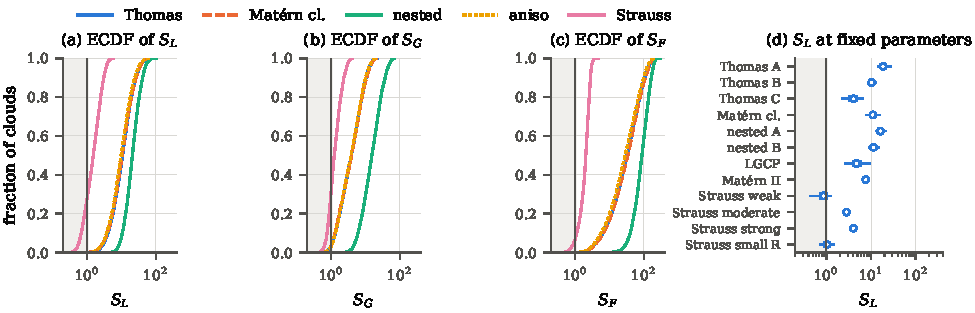
\includegraphics[width=\linewidth]{figs/fig_departure.pdf}
\caption{Departure from CSR, $S$ from (\ref{eq:S}); the shaded region $S\le1$ is indistinguishable from CSR at 5\%. (a--c) Empirical CDFs over the 7000 train/val/test clouds per process of the current data, computed from the repo's cached $L$, $F$ and $G$ curves. (d) Spread of $S_L$ across 400 replicates at fixed parameters (median, IQR, 5--95\%), for the settings of Figs.~\ref{fig:kfun} and \ref{fig:checks}.}
\label{fig:departure}
\end{figure}

\textbf{What the current data look like} \checked{} (Fig.~\ref{fig:departure}). Two findings shape everything that follows.
\begin{itemize}
  \item \emph{None of the clustered data is near CSR.} The fraction of clouds with $S_L\le1$ is 0.000 for Thomas, Mat\'ern cluster, nested and anisotropic Thomas. The 5\% quantile of $S_L$ is 3.1 for Thomas and 8.8 for nested; $S_F$ is larger still (median 32 for Thomas), and $G$ is the least sensitive (3\% of Thomas clouds have $S_G\le1$).
  \item \emph{Strauss is the opposite.} 28\% of clouds have $S_L\le1$, 67\% have $S_L\le2$, and 31\% have $S_G\le1$.
\end{itemize}
The ``adversarial'' set has the same $S$ distribution as the test pool (Kolmogorov--Smirnov $p=0.31$ for Thomas, $0.62$ for Strauss), as expected of an i.i.d.\ draw.

\textbf{Finite-sample noise.} $S$ is itself random. At fixed parameters its 5--95\% range spans a factor of 1.1--3.5, widest near CSR (Fig.~\ref{fig:departure}d). For example it runs from 2.3 to 6.6 for Thomas C and from 2.7 to 9.4 for LGCP, against a factor of 1.4 for Thomas B, and the weak Strauss setting straddles the threshold at 0.44--1.25. How to handle it:
\begin{enumerate}
  \item Use bins at least as wide as that spread, e.g.\ $S\le1$, $1$--$3$, $3$--$10$, $10$--$30$, $>30$.
  \item Where closed forms exist, also bin by the population value $S^\ast$: plug the closed-form $L$ into (\ref{eq:S}) with $n$ fixed. On current data, $\mathrm{Spearman}(S_L,S_L^\ast)=0.96$ (Thomas and Mat\'ern) and $0.95$ (nested).
  \item Report conclusions only if they hold under both binnings.
  \item Smooth $c_{0.95}(n)$ in $n$. With 200 null replicates per $n$ it carries roughly $\pm0.2$ of Monte Carlo error, judging by the scatter between neighbouring values of $n$.
\end{enumerate}

\subsection{A stratified test set}\label{sec:strat}
\textbf{Design.}
\begin{enumerate}
  \item Draw parameters from the \emph{training prior} and simulate at fixed $n$: accept only clouds with $|N-n^\ast|\le2\%$, with $n^\ast\in\{200,400,800\}$.
  \item Compute $S_L$, $S_G$ and $S_F$, and accept each cloud into its (process, bin, $n^\ast$) cell until the cell reaches its quota. For example, 200 clouds $\times$ 5 bins $\times$ 5 processes $\times$ 3 values of $n^\ast$ gives 15k clouds.
\end{enumerate}
Rejection sampling from the prior keeps the test parameters in-distribution, and fixing $n$ removes the $n(x)$ shortcut.
\textbf{The catch.} The current priors cannot fill the low bins for any clustered process (Fig.~\ref{fig:departure}). Stratifying the test set is therefore not enough. Both training and test must be regenerated from priors that reach the CSR limit (\S\ref{sec:sweeps}); otherwise every method is extrapolating in the low bins. The regeneration is cheap: clouds take minutes and diagrams are shard-parallel (\code{scripts/processing/diagrams_shard.py}).
\textbf{What to check when comparing with the old set.}
\begin{enumerate}
  \item The $S$ histograms: the i.i.d.\ set is concentrated at high $S$, while the stratified set is flat across bins by design.
  \item Reweighting stratified per-bin losses to the i.i.d.\ bin frequencies should reproduce the i.i.d.\ test loss. This is a consistency check on both.
  \item Parameter coverage per bin: which regions fill each bin (for Thomas: large $c$, small $\mu$).
  \item Class balance per bin. Classes are currently imbalanced (Thomas is 40\%) and the split is unstratified.
  \item The dependence between seed-matched Thomas and Mat\'ern twins (audit~\S5.14).
\end{enumerate}

\subsection{The analysis: performance against regime, and where classical methods fail}\label{sec:analysis}
For each method and bin, report the loss (standardised MSE; for classification, accuracy and per-class recall) together with the \emph{skill} $1-\mathrm{MSE}/\mathrm{MSE}_{\rm prior}$, where $\mathrm{MSE}_{\rm prior}$ is the loss of the prior-mean predictor. Near CSR every method regresses to the prior, and skill separates ``no information'' from ``bad model''. For confidence intervals, use a hierarchical bootstrap: resample seeds, then clouds within bins.
\textbf{Locating the threshold.} Let $\Delta(x)$ be the per-cloud paired loss difference (classical minus persistent homology). Model $\E[\Delta\mid\log S]$ with a monotone (isotonic) or segmented regression, and call $\tau^\ast$ the value of $S$ at which it crosses zero, or at which classical skill falls below a pre-registered level such as 0.5. Bootstrap the whole pipeline to get a confidence interval for $\tau^\ast$. If the band for $\Delta$ covers zero in every bin, there is no threshold to report; that is a legitimate result, and the audit's two-branch ablation (curves $0.8841$ vs.\ persistent homology plus curves $0.8836$) makes it a live possibility.
\flag \code{results.pt} stores no per-cloud predictions. This analysis needs a small code change (save test predictions and indices), or re-inference from the saved \code{model_state}.

\subsection{A regime-gated hybrid}\label{sec:hybrid}
The experts are the classical model (the $L{+}F{+}G$ CNN) and the persistent-homology model, trained as now. The gate input is label-free: $z=(\log S_L,\log S_G,\log S_F,\log n)$. Three gates:
\begin{itemize}
  \item \textbf{Hard gate}: use the persistent-homology expert if $S\le\tau$, else the classical one.
  \item \textbf{Soft gate}: $\hat y=w(z)\hat y_{\rm cl}+(1-w(z))\hat y_{\rm PH}$ with $w=\mathrm{sigmoid}(a^\top z+b)$, five parameters; mix probabilities for classification.
  \item \textbf{Learned mixture}: a small MLP on $z$ or on both embeddings.
\end{itemize}
\textbf{Fitting the gate without touching the test set.} The gate must be fitted on predictions the experts were not trained on. The cleanest way is $K$-fold cross-fitting on train+val: out-of-fold predictions from both experts on every training cloud, the gate fitted on those, the experts refitted on all of train, and the test set used once. The simpler way is to fit the gate on validation predictions and select its hyperparameters by inner cross-validation within validation. Validation has about 1050 clouds per process, so keep the gate low-dimensional.
\textbf{Baselines the claim must beat.}
\begin{enumerate}
  \item Each expert alone, with matched inputs (including $n(x)$), budgets and optimisers.
  \item \emph{Naive concatenation}: one network on both feature sets (the repo's two-branch \code{tb__PHcurves}).
  \item A constant-weight ensemble ($w$ fitted without $z$). Two diverse models almost always beat either alone, so the gate must beat plain ensembling.
  \item The same gate over two classical networks trained from different seeds, to show that the persistent-homology expert adds more than any second network.
  \item The gate with $z=\log n$ only, to test whether ``regime'' is just sample size.
  \item The oracle gate (the per-cloud best expert) as an upper bound on the headroom.
\end{enumerate}
Use paired per-cloud differences with bootstrap intervals. The Wilcoxon-over-seeds statistics must allow for cross-job non-determinism (audit~\S5.6).

\subsection{Risks and confounds}\label{sec:risks}
\begin{itemize}
\item \textbf{Circularity.} $S_L$ is a functional of the classical expert's own input, so low-$S$ bins are, by construction, the clouds where its input is flat. A persistent-homology advantage there could reflect different noise rather than different signal. Mitigations: bin by $S^\ast$; bin by a function the classical model does not see (e.g.\ $S_F$ for an $L$-only model).
\item \textbf{Identifiability.} Near CSR the parameters are weakly identified ($\gamma$ when $\pi\tau^2(1-\gamma)$ is small; $c$ as $c\to\infty$), so losses are dominated by the prior. Report skill, and check calibration.
\item \textbf{Noisy strata.} Near CSR, $S$ has an error spread of up to a factor of about 3, which brings regression to the mean. Use wide bins and cross-check with $S^\ast$ (\S\ref{sec:departure}).
\item \textbf{Prior shift.} New priors that reach CSR change what ``in-distribution'' means. Retrain everything on them and report the old i.i.d.\ numbers separately.
\item \textbf{Estimator artefacts.} $\hat\lambda^2$ absorbs clustering at small $\kappa$ (\S\ref{sec:derivK}); the Mat\'ern~II edge excess (\S\ref{sec:m2}); the LGCP thinning cap (\S\ref{sec:lgcp}).
\item \textbf{Unequal inputs and budgets} between arms (audit~\S5.4), non-determinism (\S5.6), and multiple comparisons across bins, processes and statistics. Pre-register the bins and the primary statistic ($S_L$), and apply Holm correction to the rest.
\item \textbf{Hybrid gains that are really ensembling}: baseline 3 above.
\end{itemize}

\bibliographystyle{plainnat}
\bibliography{notes}

\end{document}
